\chapter{Requirement Analysis}
\label{chapter:requirement-analysis}

In the waterfall model, as proposed by Royce, requirements analysis is typically the first phase of the development process \cite{royce70}. This phase involves gathering, documenting, and analyzing stakeholders' needs and expectations to define the software project's scope and objectives \cite{Hausen}. The objective of requirements analysis is to pinpoint the user needs and translate them into explicit, quantifiable, and attainable requirements that the software development team can employ to design and build the system \cite{Walker_2023}.

As per the findings of Walker \cite{Walker_2023}, diverse teams usually carry out this phase within a large organization. Business Analysts identify and document system needs, while Project Managers oversee the process. Developers use these requirements to design the system, and Testers validate them. Stakeholders provide essential input, and Subject Matter Experts offer specialized knowledge to help ensure the requirements are accurate and complete.

According to Geogy and Dharani \cite{Geogy2016}, one of the significant challenges in this phase is determining what needs to be constructed, as unlike other phases in development, errors in this phase can have far-reaching consequences if identified later on. They also stated that one of the primary hurdles in the requirements specification process is striking a balance between providing sufficient detail for clear understanding without overly constraining the system.

Hence, to properly define the project requirements, the following steps are taken \cite{Simplilearn_2023}:

\subsubsection{Identify Key Stakeholders and End-Users}
During the project's initial phase, it is crucial to identify the key stakeholders with significant influence and play a vital role in determining its scope. Identifying the end-users who will benefit from the product is equally important. In this project, the primary beneficiaries of the product will be the police officers and the administrators of the police department.

\subsubsection{Capture Requirements}
The subsequent steps involve obtaining input from stakeholders and end-users through various techniques. These methods may include one-on-one interviews, focus groups, use cases, and prototypes to capture their precise requirements. Each technique has its distinct purpose, from gathering detailed individual needs to envisioning the product's overall functionality.

\subsubsection{Categories Requirements}
Once requirements are gathered, they are categorized into functional and non-function requirements. This categorization ensures clarity and avoids potential confusion.

\subsubsection{Interpret and Record Requirements}
Following categorization, a process of interpretation and recording follows. This step involves assessing the feasibility, prioritizing requirements, conducting impact analyses, resolving conflicts, and ensuring precise and detailed descriptions aligned with business objectives.

After a thorough analysis, a comprehensive document detailing the requirements is created and distributed among key stakeholders, end-users, and development teams.

\subsubsection{Sign off}
A signed agreement from key stakeholders is crucial to maintain the project's scope, prevent uncontrolled expansion, and signify the final decision on requirements.

\section{Project Requirements}
\label{section:project-requirements}

Figure \ref{fig:project-requirements-1} and \ref{fig:project-requirements-2} show the result of requirement analysis process.

\begin{figure}[!ht]
    \centering
    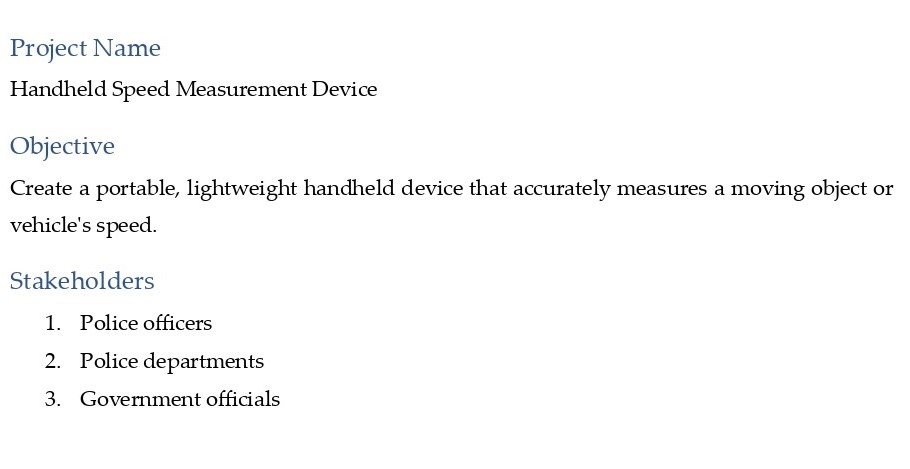
\includegraphics[width=0.9\textwidth]{texs/Part2/chapter2/image/req1.jpg}
    \caption{Project Requirements (1/2)}
    \label{fig:project-requirements-1}
\end{figure}

\begin{figure}[!ht]
    \centering
    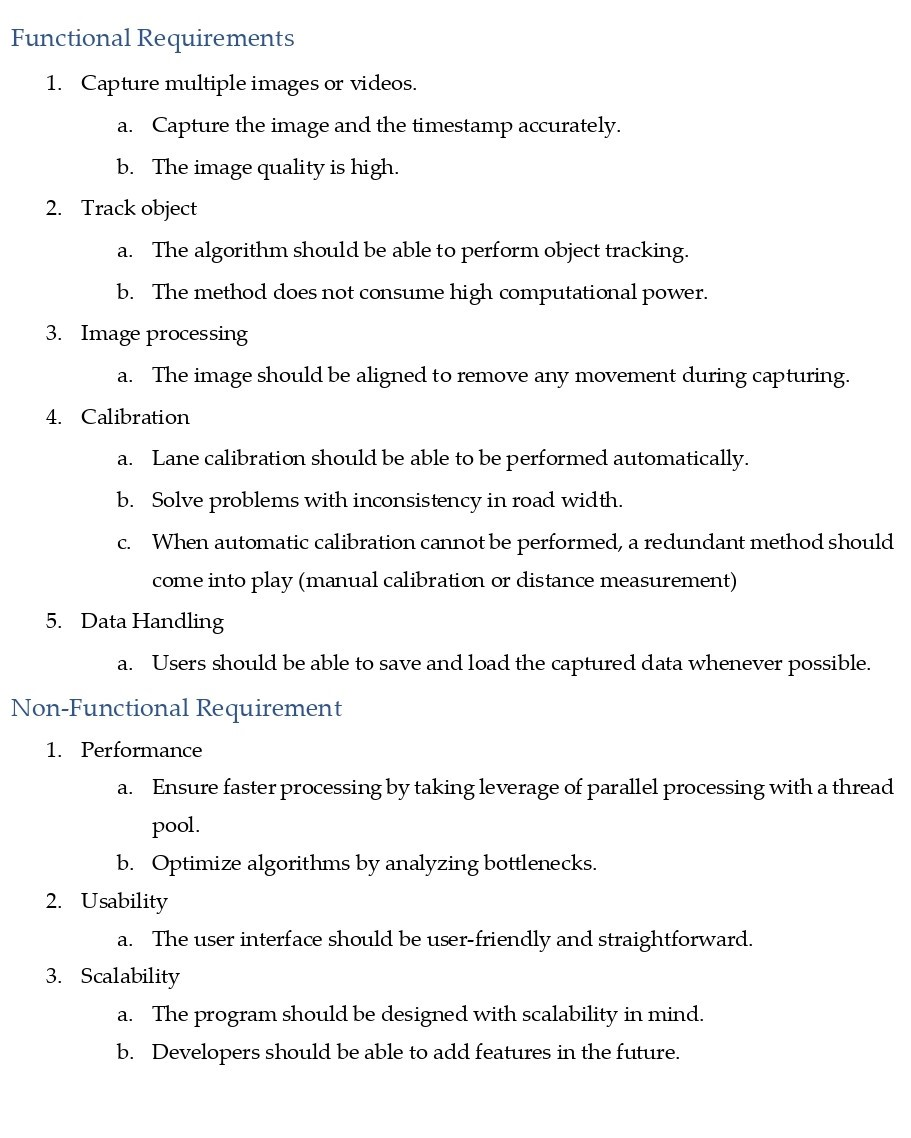
\includegraphics[width=0.9\textwidth]{texs/Part2/chapter2/image/req2.jpg}
    \caption{Project Requirements (2/2)}
    \label{fig:project-requirements-2}
\end{figure}











